\section{Number Agreement in Neural Language Models}

Neural language models have 

\begin{itemize}
    \item Describe previous results - a sparse mechanism for long-range number agreement
    \item Prediction to nested dependencies.
\end{itemize}

\begin{figure}
    \centering
    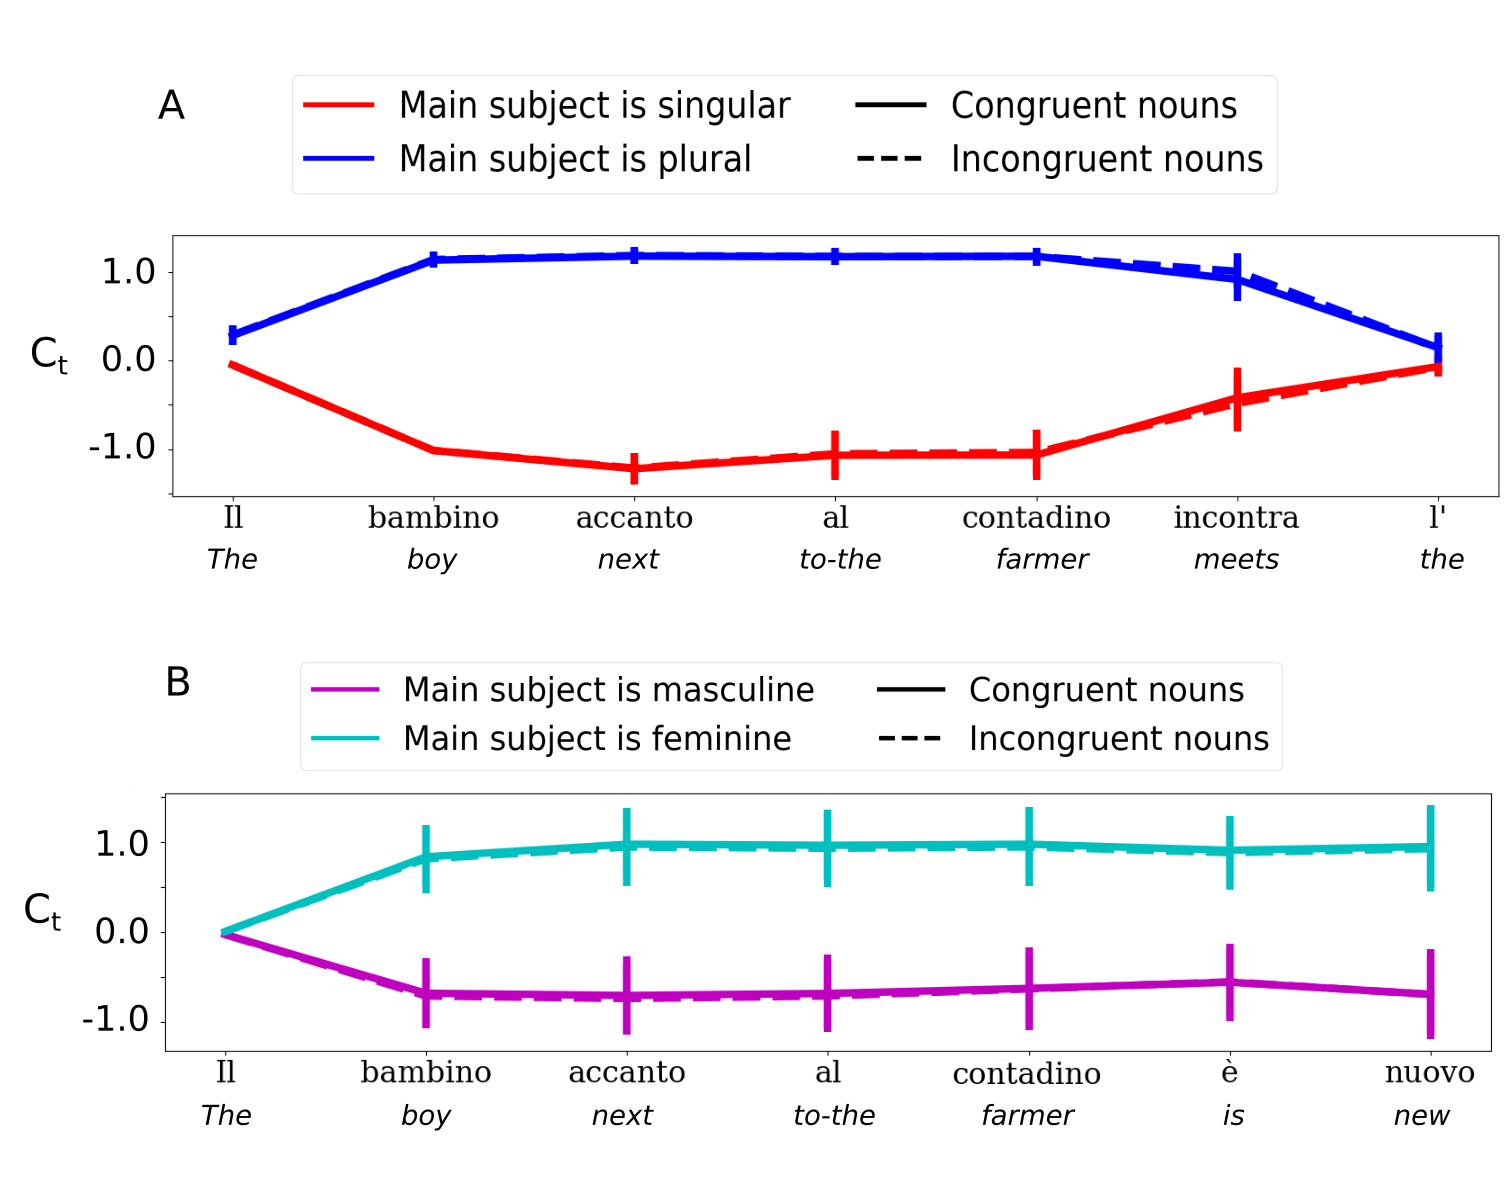
\includegraphics[width=\textwidth]{figures/model_activations_nounpp.png}
    \caption{\textbf{Cell activity of the number unit (panel A) and gender unit (panel B) during the processing of a single long-range dependency across a prepositional phrase:} four conditions are presented, corresponding to whether the main subject of the sentence is singular (red curves) or plural (blue), and to whether the main subject ('bambino') and the intervening noun ('contadino') have the same (congruent) or opposite number (incongruent)}
    \label{fig:nounpp}
\end{figure} 


\begin{figure*}
    \centering
    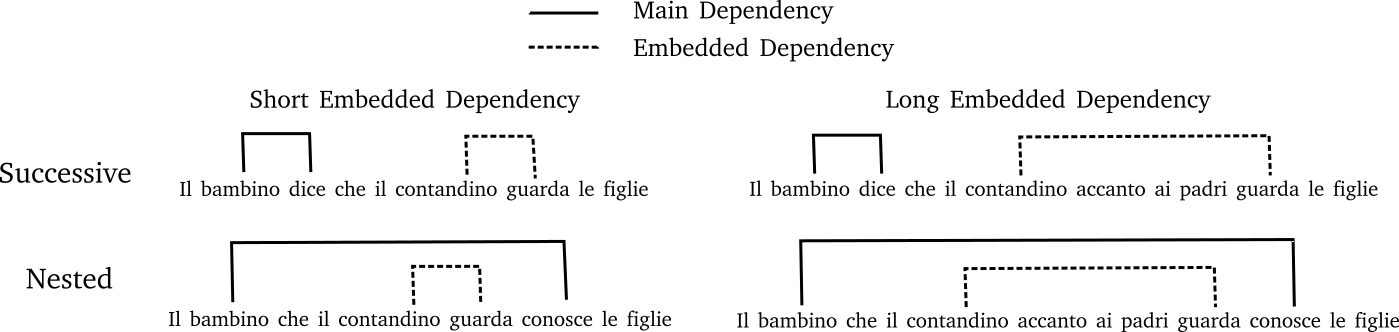
\includegraphics[width=\textwidth]{figures/design.png}
    \caption{\textbf{A full-factorial design for two subject-verb dependencies}. Human subjects and Neural Language Models (NLMs) were presented with sentences from four different syntactic structures, which all have two subject-verb dependencies: a main dependency (continuous lines) and an embedded dependency (dashed). The first factor of the design determines whether the two dependencies are \textit{successive} (top structures) or \textit{nested} (bottom), depending on whether the structure has a sentential complement (SC) or an object-extracted relative clause (objRC), respectively. The second factor determines whether the embedded dependency is \textit{short} (left side) or \textit{long} (right). We refer to the four resulting structures as: SC-short, SC-long, objRC-short and objRC-long.}
    \label{fig:design}
\end{figure*}